\section{Referencial Teórico}

O presente capítulo apresenta os conhecimentos necessários para a compreensão do presente trabalho. 

\subsection{Redes \emph{Ad Hoc}}

Uma rede \emph{ad hoc} é definida como uma coleção de entidades móveis interligados por uma tecnologia sem fio, formando uma rede temporária sem a ajuda de qualquer administração ou qualquer tipo de apoio fixo \cite{Zafoune:2007}. É um tipo descentralizado de rede, visto que não depende de uma infra-estrutura pré-existente, como roteadores em redes com fio ou pontos de acesso em redes sem fio \cite{Niazi:2009}. Outra característica é a capacidade das redes \emph{ad hoc} adequarem a condição da conectividade da rede, distribuindo a responsabilidade de organização e controle da rede para os nós, podendo determinar se um nó vai transmitir ou não dinamicamente \cite{Rezende:2008}.

As redes \emph{ad hoc} possuem características próprias que a tornam adequadas a situações onde não existe uma infra-estrutura de comunicação presente \cite{Niculescu:2003}. Elas também podem ser utilizadas em situações onde não seja possível utilizar nós críticos para organização ou controle da rede, pois o desempenho da rede \emph{ad roc} não é afetado se um nó falhar ou mesmo sair da rede \cite{Dressler:2008}.

\subsection{Redes Tolerantes a Interrupção}
Segundo \cite{Nichols:2007}, \emph{Delay-tolerant networking} (DTN) são redes projetadas para trabalhar em ambientes com comunicação instável ou temporária produzido por limitações ou anomalias, causando o menor impacto negativo possível na aplicação. 

O autor \cite{Burgess:2006} sugere que rotas instáveis podem ser causadas por problemas como: a alta mobilidade dos nós, a baixa densidade de nós, uma curta faixa para transmissão de dados ou interferências ambientais.

A DTN é uma arquitetura de rede muito utilizada atualmente na exploração do espaço ou de planetas distantes \cite{Spyropoulos:2010}, por que o espaço é um ambiente hostil que proporciona um longo período de latência no sinal, como também existe uma grande interferência eletromagnética.

 \subsection{Redes Moveis \emph{Ad Hoc}}
A \emph{Mobile Ad Hoc Networks} (MANET) é uma categoria de redes \emph{ad hoc} \cite{Rezende:2008} onde os nós são livres para deslocarem enquanto se comunicam com outros nós. Por causa da natureza dinâmica da MANET os dados que trafegam por ela podem ser corrompidos ou perdidos com facilidade \cite{Bai:2003}.

Essa configuração de rede proporciona uma frequente perda de conexão entre os nós, portanto as MANETs precisam de protocolos que possam estabelecer uma boa qualidade de serviço \cite{Bai:2003}. Essas características móveis permitem que grupos de celulares possam se conectar sem precisar de uma infraestrutura fixa somente criando uma rede \emph{ad hoc} \cite{Piorkowski:2009}.

 \subsection{Redes Veiculares Ad Hoc}



As \emph{Veicular Ad Hoc Networks} (VANET) são um conjunto de veículos que possuem capacidade computacional e estão ligados em uma rede. A VANET é um tipo de MANET que não possuem recursos limitados, então não existe a necessidade de preocupação com uso de recursos como por exemplo energia, processamento e memória \cite{Loulloudes:2010}.

A velocidade dos nós é outro fator importante no desenvolvimento de uma VANET \cite{Kumar:2011}, partindo do princípio que veículos possuem uma velocidade muito maior de deslocamento do que dispositivos móveis. 

O autor \cite{Kumar:2011} afirma que as redes veiculares podem ser construídas de três maneiras. A primeira é utilizando um modelo celular onde pontos fixos espalhados funcionam como ponte para conexão dos veículos. O segundo é uma rede onde as intersecções dos veículos são pontes para transmissão dos dados. A terceira maneira para construir uma rede rede veicular é uma técnica híbrida com a rede \emph{ad Hoc} e celular onde existem os pontos fixos e a intersecções para trafegar os dados entre os veículos. Esse modelos são exemplificados na figura \ref{fig:fig28}.

\begin{figure}[htbp]
	\centering
		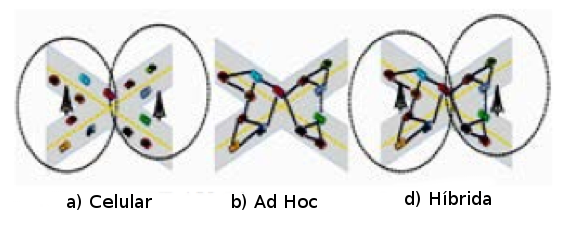
\includegraphics[scale=0.4]{referencial/figuras/Figure28.png}
	\caption{Tipos de VANET \cite{Kumar:2011}.}
	\label{fig:fig28}
\end{figure}

De acordo com \cite{Piran:2011}, com a utilização de sensores nos veículos podem ser desenvolvidos aplicações de dois tipos:

\begin{description}
\item[Aplicação para Segurança:] são utilizadas para reduzir os acidentes envolvendo veículos por exemplo monitorar velocidade, notificação de acidente, notificação de perigo na estrada e alerta de colisão.

\item[Aplicação para Segurança:] são utilizados como para o conforto dos condutor do veículos  por exemplo para notificações de roubo, de congestionamento, de multas de trânsito e informações sobre o tráfico de veículos em um determinado trajeto.
\end{description}

O desempenho de uma VANET pode ser afetado pela topologia da rede que é alterada frequentemente \cite{Lidstrom:2010}, prejudicando o desenvolvimento de aplicações em tempo real por possuir baixo nível de confiança.

\subsection{Sistemas Multi-Agentes}

Segundo \cite{Woolridge:2001}, sistemas multi-agente são sistemas compostos por agentes inteligentes com capacidade de controlar o próprio comportamento e interagir com o ambiente. O autor \cite{Woolridge:2001} sugere que os agentes podem ser agente de software, robôs ou qualquer outro tipo de recurso que realize tarefas.

De acordo com \cite{Woolridge:2001}, os agentes em um sistema multi-agente tem algumas características importantes: 

\begin{description}
\item[Autonomia:] os agentes são pelo menos parcialmente autônomos.

\item[Visão locais:] nenhum agente tem uma visão completa do sistema.

\item[Descentralização:] não há nenhum agente designado para controlar.

\end{description}

O agente possui um conjunto de tarefas para serem executadas nos nós de uma rede. Os nós possuem uma certa capacidade para realizar essas tarefas e também possuem uma quantidade limitada de recursos que podem ser utilizados pelos agentes. Para executar essas tarefas os agentes precisam percorrer a rede para poder acessar os recursos dos nós \cite{Shehory:1998}.

Para \cite{Freitas:2011}, existem duas estratégias para que o agente se locomova sobre a rede. A primeira é através da clonagem dos agentes, enquanto o segundo é chamado de migração dos agentes. Ambos os mecanismos utilizam o mesmo agente que se deslocam pelos nós em uma rede. No entanto, eles se distinguem pelo fato de o agente do primeiro cria uma cópia de si mesmo e este clone é enviado para outro nó, enquanto no segundo, o próprio agente é transmitido para outro nó.


A utilização de um sistema multi-agente sobre VANETs é interessante por que a topologia da rede está em constante mudança, sendo assim é necessário que as escolhas sejam realizadas de acordo com a organização da rede \cite{Freitas:2011}. 

Essas características de sistemas multi-agentes citadas anteriormente tornam a utilização das VANETs mais flexível.  

\subsection{Roteamento geográfico}

Roteamento Geográfico é um conceito de roteamento que se baseia em informações de posição geográfica. Essa organização é propostas para redes sem fio e com base no principio de que a fonte envia uma mensagem para a posição geográfica do destino em vez de usar o endereço de rede \cite{Shu:2010}. 

A utilização de roteamento geográfico em um VANET é sugerida em \cite{Freitas:2011} partindo do principio que o veiculo é maior e possui mais energia facilitando o transporte de um GPS.


Uma importante exigência para a implementação do roteamento geográfico é que cada nó possa determinar sua própria localização e que o emissor esteja ciente da localização do destino. Essas informações são importantes para que os dados transmitidos possam chegar ao destino \cite{Guise:2011}.

Segundo \cite{Taylor:2006}, existem duas técnicas para realizar um roteamento geográfico: 

\begin{itemize}
\item \textbf{Encaminhamento Geográfico}: é um método de roteamento que utiliza a distância geográfica entre dois nós. Os nós simplesmente transmitem pacotes de dados para o seu vizinho mais próximo até o local de destino especificado no pacote. No entanto, este esquema simples pode levar a zonas onde o nó não tem conectividade para região do alvo. 

\item \textbf{Roteamento por Perímetro}: é usado para rotear pacotes em torno das janelas encontrados na rede, assim utilizando alguns algoritmos de grafos para poder contornar essas janelas e atingir os nós que estão no destino.

\end{itemize}

\subsection{Modelo de Movimentos}

Para realizar as simulações nesse trabalho foram utilizados modelos de movimentos, que simulam o comportamento dos nós.

Os modelos de movimentos representam o movimento de componentes móveis, a mudança de sua localização, velocidade e aceleração ao longo do tempo. Tais modelos são frequentemente utilizados para fins de simulação, quando novas técnicas de navegação ou de comunicação são investigados \cite{Nichols:2007}. 

A utilização de modelos de movimentos para realizar simulações em VANET servem para simular os padrões de comportamento dos componentes da rede, por que utilizar componentes reais é inviável \cite{Freitas:2011}.

O autor \cite{Sun:2002} sugere duas abordagens para construir um modelo de movimento:

\begin{itemize}
\item \textbf{Analítico}: esse modelo de movimento é construído por uma fórmula matemática que define os padrões de comportamento dos elementos representados no modelo. 

\item \textbf{Simulado}: é construído através da observação do comportamento dos nós no ambiente que se deseja criar a simulação.

\end{itemize}

\subsection{Simulador GRUBiX}

Para desenvolvimento das técnicas de roteamento propostas neste trabalho, será utilizado o simulador de redes sem fio GRUBiX. Este simulador é uma variação do projeto SHOX \cite{Lessmann:2008}. Assim como o SHOX, o simulador GRUBiX caracteriza-se como um ambiente de simulação orientado a eventos. De forma simplificada, em um ambiente de simulação orientado a eventos, a linha do tempo de uma simulação é representada por uma lista de eventos, em que cada novo evento é inserido nesta lista. A posição em que cada evento é inserido nesta lista varia de acordo com o momento em que cada evento deve ocorrer.

Adicionalmente, estes simuladores oferece um conjunto de ferramentas para que se possa desenvolver toda a pilha de protocolos presente em um equipamento com rede sem fios. Essa disponibilidade permite que cada camada da pilha de protocolos seja personalizada de acordo com as necessidades de cada aplicação.

Assim como o SHOX, o simulador GRUBiX utiliza a linguagem de programação Java. O uso de uma linguagem orientada a objetos, nesse caso Java, indica que as camadas da pilha de protocolos sejam modeladas como objetos. O uso da orientação a objetos permite que cada camada seja personalizada através de mecanismos de herança. Portanto, basta que a nova camada personalizada herde as funcionalidade de uma camada base para que se tenha a possibilidade de alterar o seu comportamento padrão.

\subsection{Padrão ZigBee}

O ZigBee é um padrão de radio frequência que tem como objetivo a padronização e a interoperabilidade de produtos. Ele foi criado e é mantido por um grupo de empresas denominado ZigBee Alliance \cite{ZigBeeAlliance:2015}. O nome ZigBee é uma analogia da forma que as abelhas transitam entre as flores \cite{Safaric:2006}.
A especificação é a IEEE 802.15.4 na camada física e na \emph{Medium Access Control} (MAC) e para camada de rede e aplicação utiliza o ZigBee. Essa pilha pode ser observada na Figura \ref{fig:pilhaZigbee}.

\begin{figure}[htbp]
	\centering
		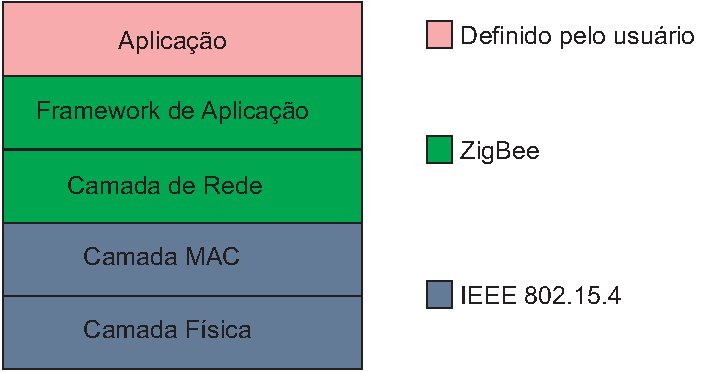
\includegraphics[scale=0.6]{referencial/figuras/pilhaZigbee.pdf}
	\caption{Pilha de protocolo ZigBee.}
	\label{fig:pilhaZigbee}
\end{figure}

O Trabalho \cite{Ramya:2011} lista como as principais características do padrão ZigBee:


\begin{itemize}
  \item Auto reparação.
  \item Suporte a muitos nós.
  \item Facilidade de implementação.
  \item Baixo consumo de energia.
  \item Padrão aberto.
\end{itemize}

\subsection{Arduíno}

O Arduíno é uma plataforma aberta composta por hardware e software. Geralmente são construídos com controladores Atmel AVR de 8 bits. O Arduino pode ser interligados a outros módulos através de hardwares denominados \emph{shields} \cite{Arduino:2015}.

Nesse trabalho é utilizado o modelo Uno \ref{fig:arduinoUno}, que possui um microcontrolador Atmel ATmega 328p com CPU operando a 16MHz. Oferece quatorze portas de entrada e saída, 32kb de memória de programa, 2Kb de SRAM e duas interrupções externas que são mapeadas pelos pinos 2 e 3 da placa. A comunicação com periféricos externos é realizada de forma serial através de uma porta USB \cite{Arduino:2015}.

\begin{figure}[htbp]
	\centering
		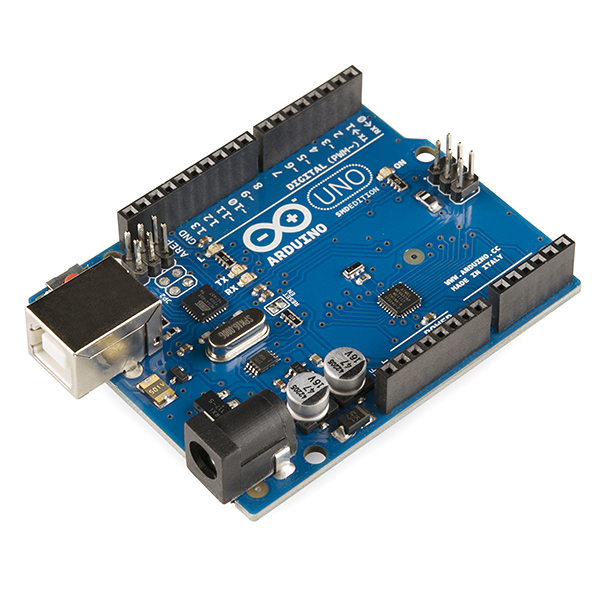
\includegraphics[scale=0.2]{referencial/figuras/arduinoUno.jpg}
	\caption{Arduino UNO.}
	\label{fig:arduinoUno}
\end{figure}

Para programar o Arduino utiliza C/C++. Ele também possui uma IDE demonstrado na Figura \ref{fig:arduinoIde}, com editor de texto e também responsável por carregar o programa na placa do Arduino.

\begin{figure}[htbp]
	\centering
		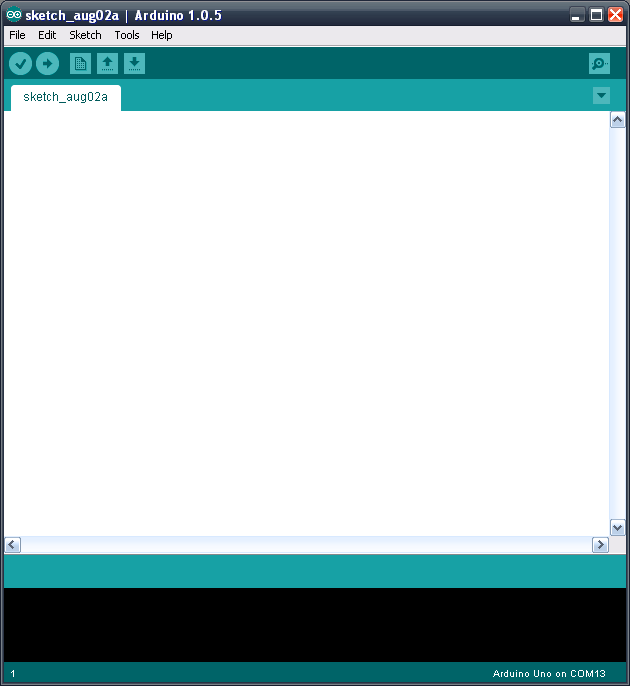
\includegraphics[scale=0.2]{referencial/figuras/arduinoIde.png}
	\caption{Arduino IDE.}
	\label{fig:arduinoIde}
\end{figure}

Para realizar a comunicação esse trabalho utiliza um \emph{shield} para integrar com o módulo Xbee denominado \emph{Xbee shield}.  

\subsection{Trabalhos relacionados}

No trabalho \cite{santanaMestrado:2014}, utiliza-se o protocolo ZigBee para desenvolver uma mecanismo para evitar colisão. O Zigbee é utilizado para enviar aos vizinhos a posição geográfica do veículo obtida através de um dispositivo android. Quando o dispositivo identifica uma possível colisão ele emite um alerta. Para identificar a colisão o disposivo utiliza a longitude e latitude do veículo, a precisão e velocidade. Essas informações são transmitidas pelos vizinhos utilizando o ZigBee.

Os testes realizados por \cite{santanaMestrado:2014} obtiveram uma latência máximo de 65 ms. Com esse resultado mostra que o padrão ZigBee atende aos requisitos de latência para rede veiculares.



O trabalho de \cite{Freitas:2011} analisa a utilização de agentes sensitivos a posição geográficas com diferentes niveis de inteligência. Nele são simulados três níveis de inteligência dos agentes. Os resultados das simulações fornecem informações sobre a importância do uso do contexto para que os agentes possam cumprir a sua missão. 

